\chapter{FISSA -- Fault Injection Simulation for Security Assessment}
\chaptermark{FISSA - Fault Injection Simulation for Security Assessment}
\label{chapter:fissa}
\minitoc

%%%%%%%%%%%%%%%%%%%%%%%%%%%%%%%%%%%%%%%%%%%%%%%%%%%%%%%%%%%%%%%%%%%%%%%%%%%%%%%%%%%%%%%%%%%%%%%
\section{Introduction}
This chapter introduces and presents a tool, called FISSA -- Fault Injection Simulation for Security Assessment --, created to automate FIAs campaigns in simulation.
This work has been published in DSD 2024~\cite{PLG-24-dsd}.
The first section presents the state of the art of existing tools for FIAs campaigns in simulation, using formal methods, or even to perform real world attacks.
The second section presents FISSA software architecture, details how FISSA works, and presents how to extend it.
The third section illustrates FISSA capacity through a use case from Section~\ref{section:uses_cases}.
Finally, the last section discusses and draws some perspectives for the tool's development and usability.

%%%%%%%%%%%%%%%%%%%%%%%%%%%%%%%%%%%%%%%%%%%%%%%%%%%%%%%%%%%%%%%%%%%%%%%%%%%%%%%%%%%%%%%%%%%%%%%
\section{Simulation tools for Fault Injection}

Addressing fault injection vulnerabilities is crucial. In general, fault attacks are conducted using physical equipment. Nonetheless, another approach exists that leverages simulators for fault testing. The main advantages of using simulators are they cost less money than physical setups, it is easier to make them work as they do not need specific skills, and they can be used during the conceptual stage.

This section presents recent works related to methods and tools for vulnerability assessment when considering FIAs. For such vulnerability assessment, main strategies include actual fault injections, formal methods and simulations.
Another objective of fault injection in simulation is to address safety~\cite{FTMLLE-21-icsrs}. Safety concerns revolve around unintended, accidental faults, with a focus on system reliability and resilience. The aim is to verify the system’s capability to detect and recover from these faults, ensuring that no catastrophic consequences occur as a result of such failures. This process is crucial for validating the robustness of safety mechanisms in place.

\begin{table}[t]
    \centering
    \footnotesize
    \caption{Fault Injection based methods for vulnerability assessment comparison}
    \label{table:FI_type_comparison}
    \setlength{\tabcolsep}{1pt}
    \begin{tabular}{@{}lccccccc@{}}
        \toprule
                          & References  & Cost                                & \begin{tabular}[c]{@{}c@{}}Control over\\fault scenarios\end{tabular}       & Scalability                         & \begin{tabular}[c]{@{}c@{}}Speed of\\ execution\end{tabular}                                      & Realism                             & Expertise \\ \midrule
        Formal Methods    & \cite{BSSMG-21-tches, ANR-18-ices, BBCFGS-19-esorics, SVPMRDKMS-24-eprint}     & \textcolor{ForestGreen}{Very low}  & \textcolor{ForestGreen}{Very high}  & \textcolor{red}{Very low}           & \textcolor{red}{Low}                                    & \textcolor{red}{Low}                & \textcolor{red}{Very high} \\
        Simulations       & \cite{BLK-23-access, HGASO-21-fdtc, AB-23-acns, fisim, AWMN-20-host,TMZHM-23-iolts,WLRTF-22-tcad,GS-21-jcrypto,HSP-21-ifs,KMD-24-ashes}     & \textcolor{ForestGreen}{Very low}       & \textcolor{ForestGreen}{Very high}  & \textcolor{red}{Low}                & \textcolor{red}{Low}/\textcolor{ForestGreen}{Moderate}  & \textcolor{ForestGreen}{Moderate}   & \textcolor{ForestGreen}{Low} \\
        Actual FIAs        & \cite{NNHRS-14-dsd,CMLCVR-11-crypto, BCNTW-06-procieee, BFP-19-tches, GBD-23-paine, CGVCBLC-22-cardis}     & \textcolor{Red}{Very high}           & \textcolor{Red}{Very low}           & \textcolor{ForestGreen}{Very high}  & \textcolor{ForestGreen}{Very high}                      & \textcolor{ForestGreen}{Very high}  & \textcolor{red}{Very high} \\
        \bottomrule
    \end{tabular}
\end{table}

Actual FIAs involve physically injecting faults into the target hardware using techniques such as variations in supply voltage or clock signal~\cite{BCNTW-06-procieee, BFP-19-tches}, laser pulses~\cite{BCNTW-06-procieee, CGVCBLC-22-cardis}, electromagnetic emanations~\cite{BCNTW-06-procieee} or X-Rays~\cite{GBD-23-paine}.
This approach offers valuable insights into the real impact of faults on hardware components.
However, a significant drawback of actual fault injections is that they demand considerable expertise to prepare the target, involving intricate setup procedures.
Additionally, this approach can only be executed once the physical circuit is available, potentially delaying the vulnerability assessment process until later stages of development.

Formal methods provide an advantage with mathematical proofs, ensuring a rigorous verification of the system's behaviour during fault injection experiments. Formal methods approaches such as~\cite{BSSMG-21-tches} allow the analysis of a circuit design in order to detect sensitive logic or sequential hardware elements. Arribas et al.~\cite{ANR-18-ices}, Barthe et al.~\cite{BBCFGS-19-esorics} and Simon et al.~\cite{SVPMRDKMS-24-eprint} present formal verification methods to analyse the behaviour of HDL implementations. However, this type of tool usually suffers from restrictions limiting its actual usage on a complete processor. Conventional formal approaches encounter scalability challenges due to limitations in verification techniques. In particular, the circuit structure it can analyse is usually limited (e.g. if there is a loop implemented in the design).

Many simulators for FIAs exist at different levels, to achieve different objectives, such as security at gate-level, cryptographic systems, study the impact of clock glitches, or even X-Ray. They can use Artificial Intelligence (AI) to enhance the detection~\cite{AB-23-acns}. Another way to simulate fault injections is to use QEMU (Quick EMUlator)~\cite{BLK-23-access,HGASO-21-fdtc,KMD-24-ashes}.
QEMU is an open-source machine that emulates the behaviour of a processor at a very fine-grain, using various optimizations to keep execution speed as close as possible to native system execution.
Bekele et al.~\cite{BLK-23-access} present a survey of QEMU-based Fault Injection techniques. After discussing the various techniques proposed in the state of the art, they classify into categories and compare them.
Fault Injections simulations can be performed at processor instructions level. Authors of~\cite{AB-23-acns} explore the impact of FIAs on software security. They evaluate four open-source fault simulators, comparing their techniques and suggest enhancing them with AI methods inspired by advances in cryptographic fault simulation. 
Arribas et al.~\cite{AWMN-20-host} introduces VerFI, a gate-level granularity fault simulator for hardware implementations. For instance, it has been used to spot an implementation mistake in ParTI~\cite{SMG-16-crypto}. However, this tool has been developed to check if implemented countermeasures can really protect against fault injection on cryptographic implementations, but it cannot evaluate components such as registers or memories.
FiSim~\cite{fisim} is an open-source deterministic fault attack simulator prototype utilising the Unicorn Framework and Capstone disassembler.
Tebina et al.~\cite{TMZHM-23-iolts} introduce Ray-Spect, a tool to simulate fault injection using parametric degradation of MOSFETs transistors, which is typical of X-ray fault injection.
Wang et al.~\cite{WLRTF-22-tcad} developed a framework for fault injection assessment at gate-level with design specific security properties.
Grycel et al.~\cite{GS-21-jcrypto} present, SimpliFI, a simulation methodology to test fault attacks on embedded software using a hardware simulation of the processor running the software. It relies on post-layout netlist simulations to study the impact of fault injection techniques such as clock glitches.

In this work, we focus on RTL simulations, which provides a controlled virtual environment for injecting faults. There are several solutions of simulations in an HDL simulator like Questasim, Vivado, etc. \textit{Behavioural} simulation is used to detect functional issues and ensuring that the design behaves as expected. \textit{Post-synthesis} simulation verifies that the synthesised netlist matches the expected functionality. \textit{Timed} simulation is used to ensure that the design meets timing requirements and can operate at the specified clock frequency. And finally, \textit{post-implementation} simulations are used to verify that the implemented design meets all requirements and constraints, including those related to the physical layout on the target.
Post-synthesis, timed, and post-implementation simulations can be more difficult to apprehend. This is because HDL synthesis alters the names of the various hardware elements, making it more difficult to find the various elements targeted in the behavioural section.
Behavioural simulation-based fault injection offers the advantage of enabling designers to test their system at the early beginning of the design cycle, providing valuable insights and uncovering potential vulnerabilities early in the development process. However, a limitation lies in the potential lack of absolute fidelity to actual conditions, as simulations might not perfectly replicate all hardware intricacies, introducing a slight risk of overlooking certain faults that could manifest in the actual hardware.

Table~\ref{table:FI_type_comparison} shows a comparison between these three methods for vulnerability assessment when considering FIAs regarding six metrics. These metrics are the financial cost of setting up the fault injection campaign, the control over fault scenarios (how configurable are the scenarios), scalability which refers to the method capacity to be applied to systems of different sizes or complexities, speed of execution of the campaign, realism of the fault injection campaign and the level of required expertise.
Table~\ref{table:FI_type_comparison} shows that no method is completely optimal. Each method has its own advantages and disadvantages and must be chosen by the designer according to the requirements and the available financial and human resources. Indeed, setting up an actual fault injection campaign requires much more expertise in this domain and also requires costly equipment, whereas setting up a simulation campaign can be easier for a circuit designer familiar with HDL simulation tools.
Table~\ref{table:FI_type_comparison} shows that simulation offers a good compromise to assess the security level of a circuit design. In particular, it provides an efficient solution for investigating security throughout the design cycle, enabling the concept of “Security by Design”.

%%%%%%%%%%%%%%%%%%%%%%%%%%%%%%%%%%%%%%%%%%%%%%%%%%%%%%%%%%%%%%%%%%%%%%%%%%%%%%%%%%%%%%%%%%%%%%%
\section{FISSA}
This section presents our open-source tool, FISSA, available on GitHub~\cite{fissa} under the CeCILL-B licence.

%%%%%%%%%%%%%%%%%%%%%%%%%%%%%%%%%%%%%%%%%%
\subsection{Main software architecture}
FISSA is designed to help circuit designers to analyse, at the early beginning of the development, the sensitivity to FIAs of the developed circuit. FISSA relies on behavioural simulations.
Figure~\ref{fig:archi_fissa} presents the software architecture of FISSA.
It consists of three different modules: \textit{TCL generator}, \textit{Fault Injection Simulator} and \textit{Analyser}. The first and third modules correspond to a set of Python classes.

\textit{The TCL generator}, detailed in Section~\ref{subsec:tcl_gen}, relies on a configuration file and a target file to create a set of parameterised TCL scripts. These scripts are tailored based on the provided configuration file and are used to drive the fault injection simulation campaign.

\textit{Fault Injection Simulator}, detailed in Section~\ref{subsec:FIS}, performs the fault injection simulation campaign based on inputs files from \textit{TCL generator} for a circuit design described through HDL files and memory initialisation files. For that purpose it relies on an existing HDL simulator such as Questasim~\cite{questasim}, Verilator~\cite{verilator}, or Vivado~\cite{vivado} to simulate the design according to the TCL script and generates JSON files to log each simulation.

\textit{The Analyser}, detailed in Section~\ref{subsec:analyser}, evaluates the outcomes of the simulations and generates a set of files that allows the designers to examine fault injection effects on their designs through various information.

\begin{figure}[ht]
    \centering
    \includegraphics[width=\textwidth, page=2]{c4_fissa/img/fissa/archi_fissa.pdf}
    \caption{Software architecture of FISSA}
    \label{fig:archi_fissa}
\end{figure}

Algorithm~\ref{algo:pseudoCodeSimuStages} shows a representation of a fault injection campaign. The algorithm requires the name(s) of the use case(s) on which the campaign will be, a set of targets (i.e. hardware elements into which a fault is to be injected), the number of bits of each target, the fault model and the injection window(s) under consideration, which identify the period(s), in a time interval between start ($\Delta_s$) and end ($\Delta_e$) in nanosecond, into which fault injections are carried out.
The number of bits for the campaign, will be called '$\kappa$', and '$\kappa_i$' the number of bits of one target.
The injection window will be used to calculate the number of cycles with the CPU period ($\varUpsilon_{cpu}$). So, the number of cycles can be determined by $nbCycles = (\Delta_e - \Delta_s) / \varUpsilon_{cpu}$.

Then, it runs a first simulation with no fault injected, which is used as a reference for comparison with the following simulations to determine end-of-simulation statuses. 
Then, for each target, each fault model and for each clock cycle within the injection window, the corresponding simulation is executed, and the corresponding logs are stored in a dedicated file.

Customising end-of-simulation statuses allows for adaptation to the specific requirements of each design assessment. To configure these statuses, adjustments need to be made either directly in FISSA's code or the HDL code. This process may involve evaluating factors such as:
\begin{itemize}
    \item hardware element content (signals, registers, \ldots),
    \item simulation time (e.g. the simulation exceeds a reference number of clock cycles),
    \item simulation's end (e.g. an assert statement introduced in the HDL code is reached)
\end{itemize}

\begin{algorithm}
    \caption{Simulated FIAs campaign pseudocode}
    \label{algo:pseudoCodeSimuStages}
    \normalsize
    \begin{algorithmic}[1]
        \Require $targets \leftarrow list(targets)$
        \Require $faults \leftarrow list(fault$\textunderscore$model)$
        \Require $windows \leftarrow list(injection$\textunderscore$windows)$
            \State $ref$\textunderscore$sims = simulate()$
            \For{$target \in targets$}
                \For{$fault \in faults$}
                    \For{$cycle \in windows$}
                        \State $logs = simulate(target, fault, cycle)$
                    \EndFor
                \EndFor
            \EndFor
    \end{algorithmic}
\end{algorithm}

%%%%%%%%%%%%%%%%%%%%%%%%%%%%%%%%%%%%%%%%%%
\subsection{Supported fault models}
\label{subsec:supported_fault_models}

A set of fault models has already been integrated into FISSA for different needs. For a given fault injection campaign, the relevant fault model is defined in the input configuration file and is applied to targets during the simulation phase.
Currently, supported fault models are:
\begin{itemize}
    \justifying
    \item \underline{target set to 0/1}: for each cycle of the injection window and for each target, we set them individually to 0 or 1, in turn exhaustively ($nbSimulations = nbCycles * nbTargets$),
    \item \underline{single bit-flip in one target at a given clock cycle}: for each cycle of the injection window, we do a bit-flip for each bit of every target exhaustively ($nbSimulations = nbCycles * \kappa$),
    \item \underline{single bit-flip in two targets at a given clock cycle}: we select one cycle and a couple of targets' bits (it can be the same target at two different bits) and we bit-flip these two bits ($nbSimulations = nbCycles * C_{2}^\kappa$; with $\kappa$, the sum of the bits of each target),
    \item \underline{single bit-flip in two targets at two different clock cycles}:  we select two different cycles and a couple of targets' bits (it can be the same target at two different bits) and we bit-flip these two bits ($nbSimulations = C_{2}^{nbCycles} * C_{2}^\kappa$),
    \item \underline{exhaustive multi-bits faults in one target at a given clock cycle}: we select one cycle and one target, and we try exhaustively each combination of bits (for example for a 2-bit target, it would be: 00, 01, 10, 11) and we set the target at each value ($nbSimulations = nbCycles * 2^{\kappa_i}$). It is worth nothing that for this fault model, we only take targets between 1 and 16 bits to avoid very big numbers of simulations as $2^{32}$ would be too long to simulate exhaustively,
    \item \underline{exhaustive multi-bits faults in two targets at a given clock cycle}: we select one cycle and two targets, and we try exhaustively each combination of bits (for example for a 2-bit target, it would be: 00, 01, 10, 11) for each target and we set them to each value (nbSimulations = $nbCycles * 2^{\kappa_{1i}}* 2^{\kappa_{2i}}$). The user must be vigilant about the size of his targets, as a register can be 32-bit or even up to 64-bit. Exhaustively testing each possible value for such large registers can be extremely time-consuming. For a 32-bit register, for example, the total number of simulations would reach $2^{32}$ (around 4 billion), which could lead to an astronomical amount of time and computational effort.
\end{itemize}

%%%%%%%%%%%%%%%%%%%%%%%%%%%%%%%%%%%%%%%%%%
\subsection{TCL Generator}
\label{subsec:tcl_gen}


\begin{lstlisting}[style=topPosition, language=json, label=code:configFile_fissa, caption=Example of a FISSA configuration file]
{
    "name_simulator": "modelsim",
    "path_tcl_generation": "PATH/",
    "path_files_sim": "PATH/simu_files/",
    "path_generated_sim": "PATH/simu_files/generated_simulations/",
    "path_results_sim": "PATH/simu_files/results_simulations/",
    "path_simulation": [ "PATH_SIMU/"],
    "prot": "wop",
    "version": 1,
    "name_reg_file_ext_wo_protect": "/faulted-reg.yaml",
    "application": ["buffer_overflow", "secretFunction", "propagationTagV2"],
    "name_results": {
        "buffer_overflow": "Buffer Overflow",
        "secretFunction": "WU-FTPd",
        "propagationTagV2": "Compare/Compute"
    },
    "threat_model": [
        "single_bitflip_spatial"
    ],
    "multi_fault_injection": 2,
    "avoid_register": [],
    "avoid_log_registers": [],
    "log_registers": [],
    "injection_window": {
        "buffer_overflow": [
            [137140, 137380]
        ],
        "secretFunction": [
            [2099100, 2099420]
        ],
        "propagationTagV2": [
            [33300, 33460]
        ]
    },
    "cycle_ref": 100,
    "cpu_period": 40,
    "batch_sim": {
        "buffer_overflow": 2000,
        "secretFunction": 2000,
        "propagationTagV2": 2000
    },
    "multi_res_files": {
        "buffer_overflow": 8,
        "secretFunction": 8,
        "propagationTagV2": 8
    }
}\end{lstlisting}

\begin{lstlisting}[style=topPosition, language=json, label=code:TargetFile_fissa, caption=Example of a FISSA target file]
---
## FETCH
FETCH:
    -
        name: /tb/top_i/core_region_i/RISCV_CORE/if_stage_i/pc_id_o_tag
        width: 1
    -
        name: /tb/top_i/core_region_i/RISCV_CORE/if_stage_i/pc_if_o_tag
        width: 1

## DECODE
DECODE:
    
## RF TAG
RF_TAG:
    
## EXECUTE
EXECUTE:
    
## CSR
CSR:
    
## Load Store Unit
LSU:
...\end{lstlisting}

The \textit{TCL Generator} is used to generate the set of TCL script files which drive the \textit{fault injection simulator}. This module requires two input files.
Figure~\ref{fig:archi_tcl_gen} details the \textit{TCL Generator} software architecture. Each blue box represents a python class used to generate the set of output TCL scripts.
The \textit{initialisation} class gets inputs from a configuration file. This JSON-formatted file includes various parameters such as the targeted HDL simulator, the considered fault model and the injection window(s). Furthermore, it encompasses parameters such as the clock period (in ns) of the HDL design and the maximum number of simulated clock cycles used to stop the simulation in case of divergence due to the injected fault. Moreover, one extra parameter defines the quantity of simulations per TCL file, allowing a simulation parallelism degree.
Listing~\ref{code:configFile_fissa} shows an extract of a configuration file used for our fault injection campaigns.
Listing~\ref{code:TargetFile_fissa} shows an extract from a target file according to the configuration file provided previously. This file lists each stage of the RISC-V core, and for each the HDL path of our targets are written. Here, in this example, only the list of targets for the \textit{instruction fetch} stage is listed.

The \textit{Targets} file contains, in YAML format, the list of the circuit elements (e.g. registers or logic gates) that need to be targeted during the fault injection campaign. For each target, its HDL path and bit-width are specified.
\textit{TCL Script Generator} class gets the configuration parameters from \textit{Initialisation} class, reads the \textit{Targets'} file and calls three others classes.
The first one, \textit{Basic Code Generator}, undertakes the fundamental generation of TCL code for initialising a simulation, running a simulation, and ending a simulation.
The second one, \textit{Fault Generator}, produces the TCL code related to fault injection. The \textit{TCL Script Generator} provides specific parameters to the \textit{Fault Generator} to produce code for a designated set of targets and a specified set of clock cycles for fault injection.
The third one, \textit{Log Generator}, produces the TCL code to produce logs after each simulation.
Logs comprise the simulation's ID, fault model, faulted targets, injection clock cycle(s), end-of-simulation status, values for all targets, and the end-of-simulation clock cycle. This data constitutes the automated aspect of logging.
Finally, the \textit{TCL Script Generator} outputs a set of TCL files, each one corresponds to a batch of simulations. This allows the user to perform a per batch results analysis. It is worth noting that each batch starts with a reference simulation, which means a simulation without any fault injected. This approach allows for obtaining comparative results after a fault has occurred, making it possible to determine the specific effects and consequences of the injected fault. By comparing the system's behaviour before and after the fault injection, it becomes easier to identify what was impacted and how the fault influenced the system's operation.

\begin{figure}[ht]
    \centering
    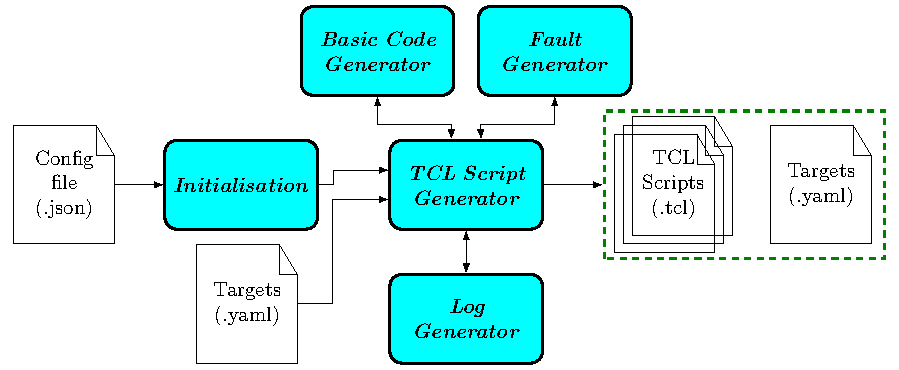
\includegraphics[width=\textwidth]{c4_fissa/img/fissa/archi_tcl_gen.pdf}
    \caption{Software architecture of the TCL Generator module}
    \label{fig:archi_tcl_gen}
\end{figure}

Algorithm~\ref{algo:pseudoCodeSimus} depicts the pseudocode of a simulation of a fault injection, showcasing requirements, and each state with essential parameters. Additionally, the corresponding Python class from Figure~\ref{fig:archi_tcl_gen} is added for each line.
Line 5 in Algorithm~\ref{algo:pseudoCodeSimuStages} corresponds to Algorithm~\ref{algo:pseudoCodeSimus}. This algorithm is executed multiple times with different inputs to build a TCL script.


\begin{algorithm}
    \caption{FIAs simulation pseudocode}
    \label{algo:pseudoCodeSimus}
    \normalsize
    \begin{algorithmic}[1]
        \Require $target$
        \Require $cycle$
        \Require $fault$\textunderscore$model$
        \State $tcl$\textunderscore$script = init$\textunderscore$sim(fault$\textunderscore$model, cycle, target)$ \textcolor{blue}{\scriptsize // generated by Basic Code Generator}
        \State $tcl$\textunderscore$script += inject$\textunderscore$fault(fault$\textunderscore$model)$  \textcolor{red}{\scriptsize // generated by Fault Generator}
        \State $tcl$\textunderscore$script += run$\textunderscore$sim()$ \textcolor{blue}{\scriptsize // generated by Basic Code Generator}
        \State $tcl$\textunderscore$script += log$\textunderscore$sim(fault$\textunderscore$model)$ \textcolor{ForestGreen}{\scriptsize // generated by Log Generator}
        \State $tcl$\textunderscore$script += end$\textunderscore$sim()$ \textcolor{blue}{\scriptsize // generated by Basic Code Generator}
        \State $tcl$\textunderscore$file.write(tcl$\textunderscore$script)$ \textcolor{black}{\scriptsize // append and write the simulation data inside the TCL file}
    \end{algorithmic}
\end{algorithm}

%%%%%%%%%%%%%%%%%%%%%%%%%%%%%%%%%%%%%%%%%%
\subsection{Fault Injection Simulator}
\label{subsec:FIS}

The \textit{Fault Injection Simulator} (Figure~\ref{fig:archi_fis}) mainly relies on an existing HDL simulator to perform simulations by executing the TCL scripts produced by the \textit{TCL generator}. The log files, in JSON format, are generated by the TCL script for each simulation.
This file encompasses data such as the current simulation number, the executed clock cycle count, the values of the targets' file, the targets faulted, the fault model and the end-of-simulation status.

Listing~\ref{code:logJSONFile_fissa} shows a simplified example of an output file from a simulation. Many lines are omitted to simplify the text and its comprehension. In this example, we have the result of the first simulation of the campaign. The fault model is a single bit-flip in one target at a given clock cycle, and the target, which is a register in this case, \texttt{pc\_id\_o\_tag}, has a size of one bit. A fault has been injected at the period time of \SI{137140}{\nano\second}. The omitted lines, at line 7, include all registers from the register file, all register file tags, and all registers from the target list. The last line, line 14, shows that this simulation ended with a status equal to 3 (i.e., exception delayed from the reference simulation).

\begin{figure}[ht]
    \centering
    \includegraphics[width=.5\textwidth, page=4]{c4_fissa/img/fissa/archi_fissa.pdf}
    \caption{Fault injection simulator architecture}
    \label{fig:archi_fis}
\end{figure}

It is worth noting that the set of calls to the generated TCL scripts has to be integrated into the designer's existing design flow, allowing the design compilation, initialisation, and management of input stimuli. The use of TCL scripts simplifies such an integration. 
Once all the fault injection simulations have been performed, the log files can be sent to the \textit{Analyser} which, is described in the following subsection.

\begin{lstlisting}[style=topPosition, language=json, label=code:logJSONFile_fissa, caption=Extract of an example of a FISSA output log JSON file]
"simulation_1": {
    "cycle_ref": 100,
    "cycle_ending": 4,
    "TPR": "32'h0000a8a2",
    "TCR": "32'h00341800",
    "rf1": "32'h000006fc",
    (...)
    "faulted_register": "/tb/top_i/core_region_i/RISCV_CORE/if_stage_i/pc_id_o_tag",
    "size_faulted_register": 1,
    "threat": "bitflip",
    "bit_flipped": 0,
    "cycle_attacked": "137140 ns",
    "simulation_end_time": "137300 ns",
    "status_end": 3
}\end{lstlisting}

%%%%%%%%%%%%%%%%%%%%%%%%%%%%%%%%%%%%%%%%%%
\subsection{Analyser}
\label{subsec:analyser}

The \textit{Analyser} (Figure~\ref{fig:archi_analyser}) reads all log files and generates a set of \LaTeX~tables (\textit{.tex} files) and/or sensitivity heatmaps (in PDF format) according to the fault models, allowing the user to identify the sensitive hardware elements in the circuit design. 
The generated tables can be customised through modification in the \textit{Analyser} Python code.
The current configuration captures and counts the diverse end-of-simulation status.
Heatmaps are generated for multi-target fault models. For instance, when considering a 2 faults scenario disturbing two hardware elements, a 2-dimension heatmap allows the user to identify sensitive couples of hardware elements leading to a potential vulnerability.
Their configuration can be adapted by modifying the \textit{Analyser} Python code. Heatmaps generation is based on \textit{Seaborn}~\cite{seaborn} which relies on \textit{Matplotlib}~\cite{matplotlib}. This library provides a high-level interface for drawing attractive and informative statistical graphics and save them in different formats like PDF, PNG, etc.
In the current configuration, heatmaps highlight the targets leading to a specific end-of-simulation status (e.g. a status identified by the designer as a successful attack).
Once the results have been generated, they can easily be inserted into a vulnerability assessment report. 

\begin{figure}[ht]
    \centering
    \includegraphics[width=.5\textwidth, page=5]{c4_fissa/img/fissa/archi_fissa.pdf}
    \caption{Analyser architecture}
    \label{fig:archi_analyser}
\end{figure}

%%%%%%%%%%%%%%%%%%%%%%%%%%%%%%%%%%%%%%%%%%
\subsection{Extending FISSA}

In order to extend FISSA for integrating an additional fault model, some modifications to the \textit{TCL Script Generator}, the \textit{Basic Code Generator}, the \textit{Fault Generator} and \textit{Log Generator} modules are necessary. 
It requires the extension of the \textit{init\_sim}, \textit{inject\_fault} and \textit{log\_sim} functions presented in Algorithm~\ref{algo:pseudoCodeSimus} to implement the new fault model from initialisation to logging. 
For instance, these extensions should define the targets for each simulation, the impact of the injections (set to 0/1, bit-flip, random, etc) and the set of data to be logged for this fault model.
The \textit{Log Generator} automates the extraction of specific segments from the ongoing simulation. However, it is customisable, enabling the modification of logged elements, such as incorporating memory content or a list of signals.

\textit{Analyser} can be extended to produce additional \LaTeX~tables, heatmaps or any other way of results visualisation. This can be achieved by either modifying the existing methods or by developing new ones.

An integral aspect of expanding FISSA involves adjusting functions depending on the used HDL simulator. Despite the definition of the TCL language, specific commands vary between simulators. For instance, in Questasim, injecting a fault into a target can be accomplished with the command: “\textit{force \textless object\_name\textgreater \textless value\textgreater -freeze -cancel \textless time\_info\textgreater}”~\cite{modelsim-force}, whereas in Vivado, the equivalent command is: “\textit{add\_force \textless hdl\_object\textgreater \textless values\textgreater -cancel\_after \textless time\_info\textgreater}”~\cite{vivado-force}.
There are some subtle differences between these two software applications that need to be taken into consideration in order to extend FISSA. These distinctions may affect the functionality or compatibility, so addressing them is crucial for a successful adaptation.

%%%%%%%%%%%%%%%%%%%%%%%%%%%%%%%%%%%%%%%%%%%%%%%%%%%%%%%%%%%%%%%%%%%%%%%%%%%%%%%%%%%%%%%%%%%%%%%
\section{Use case example}
\label{section:exampleApplication_fissa}
This section presents a case study to demonstrate the use of FISSA in real conditions. It focuses on the evaluation of the robustness of the DIFT mechanism integrated in the D-RI5CY processor with the Buffer overflow use case from Section~\ref{section:uses_cases}.

%%%%%%%%%%%%%%%%%%%%%%%%%%%%%%%%%%%%%%%%%%
\subsection{FISSA's configuration}
\label{subsec:tool_config}

This subsection presents FISSA's configuration for the addressed use case. We have defined four end-of-simulation statuses, which will be utilised to automatically generate results tables. Examples of these tables will be provided in Subsection~\ref{subsec:results}.
The initial status is labelled as a \textit{crash} (status 1), indicating that the fault injection has caused a deviation in program flow control, leading the processor to execute instructions different from those expected.
The second status, identified as a \textit{silent} fault (status 2), signifies that a fault has occurred but has not impacted the ongoing simulation behaviour.
Status 3, termed a \textit{delay}, denotes that the fault has delayed the DIFT-related exception, meaning the exception is not raised at the same clock cycle as in the reference simulation.
The last status refers to a \textit{success} (status 4), indicating a bypass of the DIFT mechanism and thereby marking a successful attack. This status corresponds to the detection of the end of the simulated program, with no exception being raised.

In the input configuration file, a single injection window is set between cycles 3428 and 3434, the maximum number of simulated clock cycles is set to 100 from the start of the injection window, this allows us to detect if there were a control flow deviation, the design period is set to 40~ns, the number of simulations per TCL script is set to 2,200. The considered fault models are four of the seven fault models defined in Section~\ref{subsec:supported_fault_models}: \textit{target set to 0}, \textit{target set to 1}, \textit{single bit-flip in one target at a given cycle}, and \textit{single bit-flip in two targets at a given cycle}.

Four FIAs simulation campaigns are performed to evaluate the design against the four fault models.
We choose to log the values of the \textit{Targets'} file, the simulation's number, targets' value after the injection, the injection cycle and the end-of-simulation status.
The \textit{Targets'} file is filled with the 55 registers of the DIFT security mechanism, representing a total of 127 bits.

%%%%%%%%%%%%%%%%%%%%%%%%%%%%%%%%%%%%%%%%%%
\subsection{Experimental results} 
\label{subsec:results}

\begin{figure}[t]
    \centering
    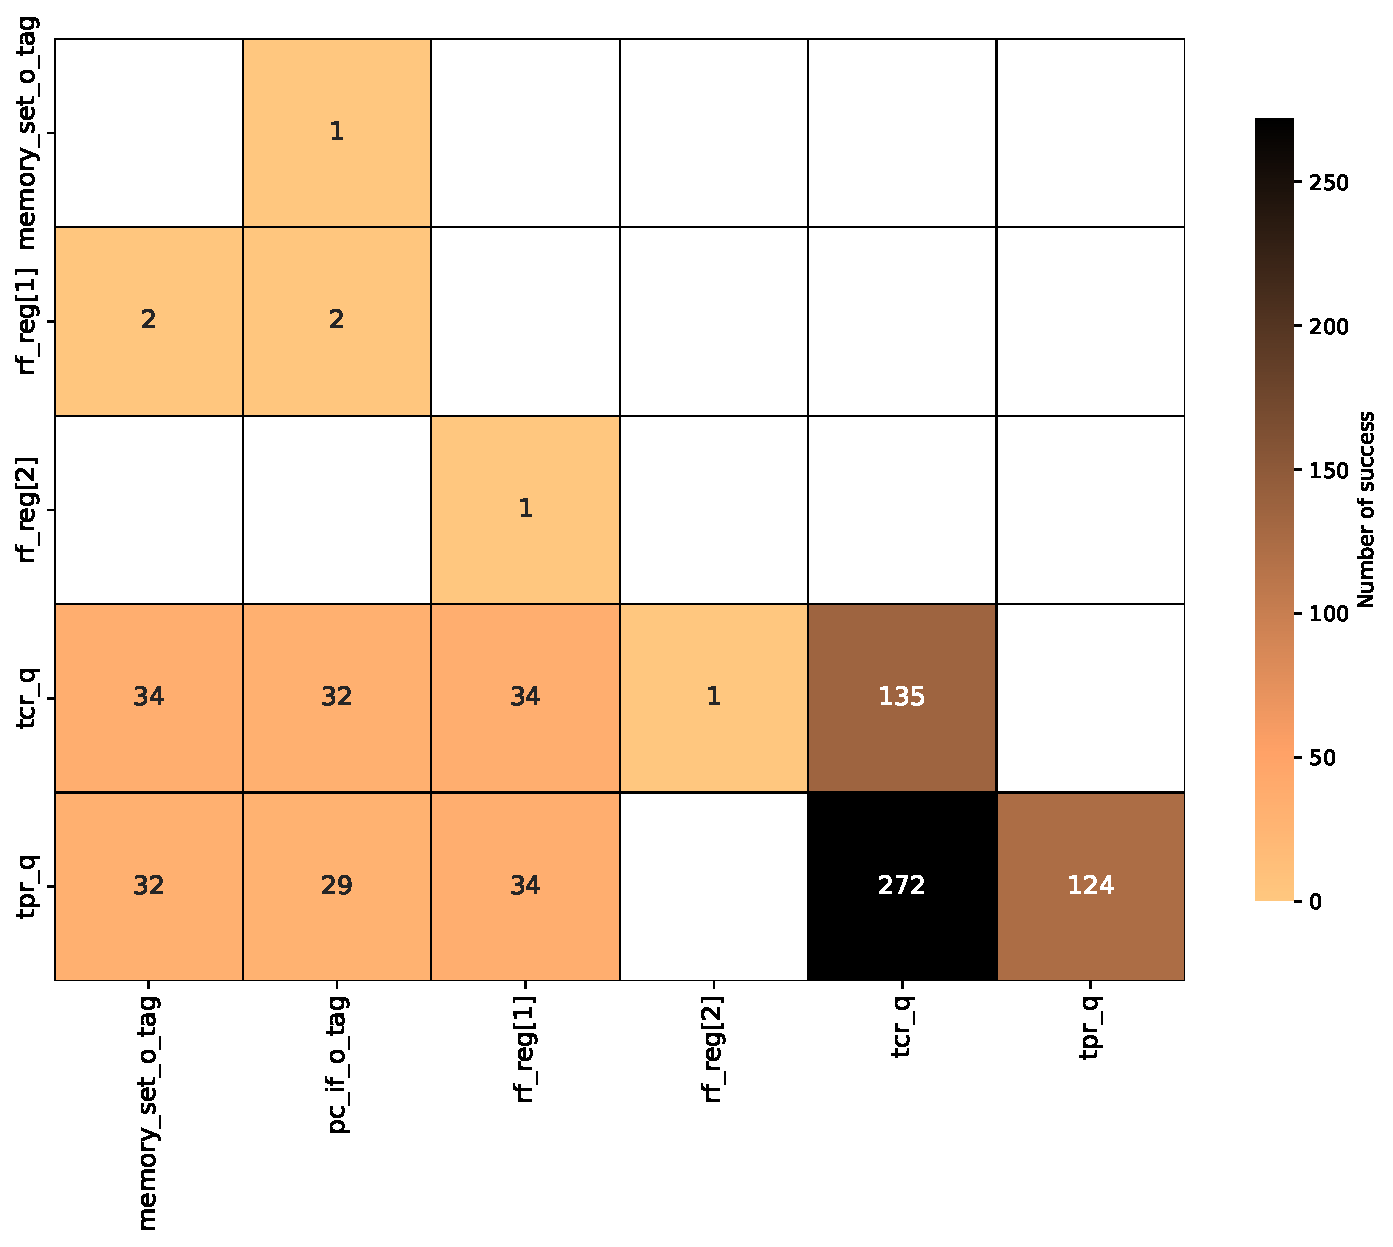
\includegraphics[width=.95\textwidth]{c4_fissa/img/heatmap/heatmap_buffer_overflow_wop_1_single_bitflip_spatial_2.pdf}
    \caption{Extract of the heatmap generated according to the single bit-flip in two targets at a given clock cycle fault model}
    \label{fig:heatmap_spatial}
\end{figure}

This section presents results obtained using FISSA on the considered use case.
All experiments are performed on a server with the following configuration: Xeon Gold 5220 (2,2~GHz, 18C/36T), 128~GB RAM, Ubuntu 20.04.6 LTS and Questasim 10.6e.

Table~\ref{table:end_sim_by_status} summarises the outcomes of the four previously described fault injection campaigns, with each row representing a distinct fault model. Table~\ref{table:end_sim_by_status}'s columns delineate the potential end statuses for each simulation. This table is an essential tool for the designers, enabling them to analyse the vulnerabilities associated with each fault model within their design. Consequently, the designers can determine the necessity for additional protective measures or design alterations.

For instance, Table~\ref{table:end_sim_by_status} illustrates that the '\texttt{set to 1}' fault model results in only three successful outcomes, which represent 0.91\% of the total number of simulations, whereas the '\texttt{single bit-flip in two targets at a given clock cycle}' fault model leads to 1,406 successes, which represent 2.93\% of the total number of simulations. These findings guide the designers in evaluating the significance of protecting against specific fault models.

To further assess vulnerabilities, the designers can utilise Table~\ref{table:end_sim_by_status_wop_1_detail_set0_set1_bitflip}, which provides detailed information on the register and cycle locations of faults for models with fewer successful outcomes. For fault models with multiple registers faulted or with a high number of successes, where the table may become unwieldy, Figure~\ref{fig:heatmap_spatial} serves as a more accessible reference. This figure helps in visualising and interpreting the spatial distribution of vulnerabilities effectively.

\begin{table}
    \centering
    \footnotesize
    \caption{Results of fault injection simulation campaigns}
    \label{table:end_sim_by_status}
    \setlength{\tabcolsep}{3pt}
    \begin{tabular}{@{}rcccccc@{}}
        \toprule
        Fault model                                                        & Crash & Silent  & Delay & Success        & Total   & \begin{tabular}[c]{@{}c@{}}Simulation\\ time\end{tabular} \\
        \midrule
        Set to 0                                                           & 0     & 320     & 1     & 9 (2.73\%)     & 330     & 0h04            \\%\hdashline
        Set to 1                                                           & 0     & 320     & 7     & 3 (0.91\%)     & 330     & 0h04            \\%\hdashline
        Single bit-flip in one target at a given clock cycle               & 0     & 738     & 12    & 12 (1.57\%)    & 762     & 0h11            \\%\hdashline
        Single bit-flip in two targets at a given clock cycle              & 0     & 45,097  & 1,503 & 1,406 (2.93\%) & 48,006  & 13h43           \\%\hdashline
        % \begin{tabular}[c]{@{}r@{}}Single bit-flip in two targets\\ at two different clock cycles\end{tabular}       & 0     & 238,633 & 1,143 & 2,159 (0.89\%) & 241,935 & 42h12           \\\hdashline
        % \begin{tabular}[c]{@{}r@{}}Exhaustive multi-bits faults in\\ one target at a given clock cycle\end{tabular}  & 0     & 927     & 6     & 3 (0.32\%)     & 936     & 0h08            \\\hdashline
        % \begin{tabular}[c]{@{}r@{}}Exhaustive multi-bits faults\\ in two targets at a given clock cycle\end{tabular} & 0     & 67,072  & 926   & 450 (0.66\%)   & 68,448  & 11h11           \\
        \bottomrule
    \end{tabular}
\end{table}

\begin{table*}[t]
    \centering
    \footnotesize
    \caption{Buffer overflow: success per register, fault type and simulation time}
    \label{table:end_sim_by_status_wop_1_detail_set0_set1_bitflip}
    \setlength{\tabcolsep}{1pt}
    \begin{tabular}{@{}rccccccccccccccc@{}}
        \toprule
                                        & \multicolumn{3}{c}{Cycle 3428}                & \multicolumn{3}{c}{Cycle 3429}             & \multicolumn{3}{c}{Cycle 3430} & \multicolumn{3}{c}{Cycle 3431} & \multicolumn{3}{c}{Cycle 3432}                                                                                                                 \\\cmidrule(lr){2-4}\cmidrule(lr){5-7}\cmidrule(lr){8-10}\cmidrule(lr){11-13}\cmidrule(lr){14-16}
                                        & set 0          & set 1          & bit-flip       & set 0          & set 1          & bit-flip    & set 0          & set 1 & bit-flip    & set 0          & set 1 & bit-flip    & set 0          & set 1 & bit-flip    \\
        \midrule
        pc\_if\_o\_tag                  &               &               &               &               &               &            &            &      &            & \checkmark &      & \checkmark &            &      &            \\
        memory\_set\_o\_tag             &               & \checkmark    & \checkmark    &               &               &            &            &      &            &            &      &            &            &      &            \\
        rf\_reg[1]                      &               &               &               &               &               &            & \checkmark &      & \checkmark &            &      &            &            &      &            \\
        tcr\_q                          & \checkmark    &               &               & \checkmark    &               &            & \checkmark &      &            & \checkmark &      &            & \checkmark &      &            \\
        \rowcolor{LightGray} tcr\_q[21] &               &               & \checkmark    &               &               & \checkmark &            &      & \checkmark &            &      & \checkmark &            &      & \checkmark \\
        tpr\_q                          & \checkmark    & \checkmark    &               & \checkmark    & \checkmark    &            &            &      &            &            &      &            &            &      &            \\
        \rowcolor{LightGray} tpr\_q[12] &               &               & \checkmark    &               &               & \checkmark &            &      &            &            &      &            &            &      &            \\
        \rowcolor{LightGray} tpr\_q[15] &               &               & \checkmark    &               &               & \checkmark &            &      &            &            &      &            &            &      &            \\
        \bottomrule
    \end{tabular}
\end{table*}

Table~\ref{table:end_sim_by_status_wop_1_detail_set0_set1_bitflip} is produced by FISSA and details the successes from three distinct fault injection campaigns: \texttt{set to 0}, \texttt{set to 1} and \texttt{single bit-flip in one target at a given cycle}. Table~\ref{table:end_sim_by_status_wop_1_detail_set0_set1_bitflip} specifies successes for each fault model, correlated with the cycle and the affected target. For example, a \texttt{set to 0} fault at cycle 3428 on \texttt{tcr\_q} would lead to a successfully attack. It highlights which targets are sensitive to fault attacks at a cycle-accurate and bit-accurate level, providing the designers precise information on critical elements requiring protection based on their specific needs.  Table~\ref{table:end_sim_by_status_wop_1_detail_set0_set1_bitflip} only covers the most basic fault models. Indeed, producing a table for more complex scenarios, such as simultaneous faults in two targets within a same or multiple cycles, would be intricate and challenging to interpret. Consequently, we opted for an alternative method and developed a heatmap representation (e.g. Figure~\ref{fig:heatmap_spatial}).

To further explore the impact of FIAs on a design, a designer can study heatmaps generated by FISSA. 
These heatmaps are tailored to a fault model with two faulty registers, where each matrix intersection shows the number of successes with that target pair.

Figure~\ref{fig:heatmap_spatial} shows an extract of the heatmap generated for the \textit{single bit-flip in two targets at a given clock cycle} fault model. For simplicity, only 5 registers are represented. The full figure will be presented in Chapter~\ref{chapter:exp_setup_results}.
The colour scale represents the number of fault injections targeting a couple of hardware elements (i.e. registers for this use case) leading to a \textit{success} as defined in Subsection~\ref{subsec:tool_config}. We can note that this colour scale, in our case, range from 0 to 272.
This figure highlights the registers that are critical to a specific fault model, enabling the designer to evaluate the design and determine where protection is needed and at what level. It provides a clear indication of which areas require minimal protection and which ones demand a very high level of security. All of this information allow the designer to prioritise countermeasures according to allocated budget, protection requirements, etc.
To give an example, it can be noted that the horizontally displayed registers \texttt{tcr\_q} and \texttt{tpr\_q} are critical registers, because a success will occur regardless of the associated register. Similarly, the registers shown vertically, \texttt{memory\_set\_o\_tag}, \texttt{pc\_if\_o\_tag}, and \texttt{rf\_reg[1]}, are also critical because they lead to many successes with almost all tested registers.

To provide an analytical perspective from the buffer overflow use case presented in Section~\ref{section:uses_cases}, the five previously mentioned registers are critical as they either store the DIFT security policy configuration (\texttt{tpr\_q} and \texttt{tcr\_q}) or store (\texttt{rf\_reg[1]} represents the tag associated with the value of the Program Counter (PC), which is stored in the register file at index 1 for RISC-V ISA) and propagate the tag (\texttt{pc\_if\_o\_tag}) associated with the PC. This is particularly important in our example, which demonstrates a ROP attack with a buffer overflow.
The colour scale indicates the impact of the fault injections on the combination of registers tested. For example, a pair associated with a high number such as 272, 124, and 135 for \texttt{tcr\_q} and \texttt{tpr\_q} are very high priority as they lead to 37.77\% success on this fault model (i.e. with all registers taken into account, see Table~\ref{table:end_sim_by_status}).
In addition, we can see that a register produces a low number of successes, such as \mbox{\texttt{rf\_reg[2]}}; this register is then not the highest priority for protection for the designer.

While Table~\ref{table:end_sim_by_status} provides the total number of \textit{successes} for each fault model and Table~\ref{table:end_sim_by_status_wop_1_detail_set0_set1_bitflip} gives the successes for each fault model (\textit{set to 0}, \textit{set to 1}, and \textit{a single bit flip in a target at a given cycle}) correlated with the cycle and affected target, Figure~\ref{fig:heatmap_spatial} shows that fault injections in 246 register pairs result in a \textit{success}. This information allows the designer to focus on specific simulation traces to understand the effect(s) of the fault(s) and improve the robustness of his design by implementing adapted countermeasures.

%%%%%%%%%%%%%%%%%%%%%%%%%%%%%%%%%%%%%%%%%%%%%%%%%%%%%%%%%%%%%%%%%%%%%%%%%%%%%%%%%%%%%%%%%%%%%%%
\section{Discussion and Perspectives}

In this section, we will discuss this proposed tool and draw some perspectives.
In terms of execution time, we did in total around 24,000,000 simulations for approximatively 3 seconds for each simulation in average spanning from initialisation to data recording.
The execution time is contingent upon various parameters, including the design's size, the specific simulation case, and the number of targets involve.
Actual FIAs are faster than simulations, taking about 0.35 seconds per injection in our tests, relying on the ChipWhisperer-lite platform for clock glitching injection.
While simulations may be slower, they offer the benefit of not requiring an FPGA prototype or the final circuit. Furthermore, it allows integrating vulnerability assessment in the first stages of the development flow and provides a rich set of information for the designer in order to understand sources of vulnerabilities in his design.

As perspectives, we plan to extend FISSA to support new fault models and HDL simulators such as Vivado or Verilator.
Additionally, we intend to enhance integration into the design workflow by adding more automation. This may include the management of HDL sources compilation, design's input stimuli or the development of a graphical user interface to improve the overall user experience.
%%%%%%%%%%%%%%%%%%%%%%%%%%%%%%%%%%%%%%%%%%%%%%%%%%%%%%%%%%%%%%%%%%%%%%%%%%%%%%%%%%%%%%%%%%%%%%%
\section{Summary}
In this chapter, we presented FISSA (Fault Injection Simulation for Security Assessment), our advanced and versatile open-source tool designed to automate fault injection campaigns. FISSA is engineered to seamlessly integrate with renowned HDL simulators, such as Questasim. It facilitates the execution of simulations by generating TCL scripts and produces comprehensive JSON log files for subsequent security analysis.

FISSA empowers designers to evaluate their designs during the conceptual phase by allowing them to select specific assessment parameters, including the fault model and target components, tailored to their unique requirements. The insights gained from the results generated by this tool enable designers to enhance the security of their designs, thus adhering to the principles of \textit{Security by Design}.


%%%%%%%%%%%%%%%%%%%%%%%%%%%%%%%%%%%%%%%%%%%%%%%%%%%%%%%%%%%%%%%%%%%%%%%%%%%%%%%%%%%%%%%%%%%%%%%